% ==============================================================================
% DevOS Architecture Diagram - TikZ Source
% Compile with: pdflatex architecture.tex
% Or include directly in main.tex using \input{figures/architecture}
% ==============================================================================

\documentclass[tikz,border=10pt]{standalone}
\usepackage{tikz}
\usetikzlibrary{shapes, arrows.meta, positioning, calc, fit, backgrounds}

\begin{document}

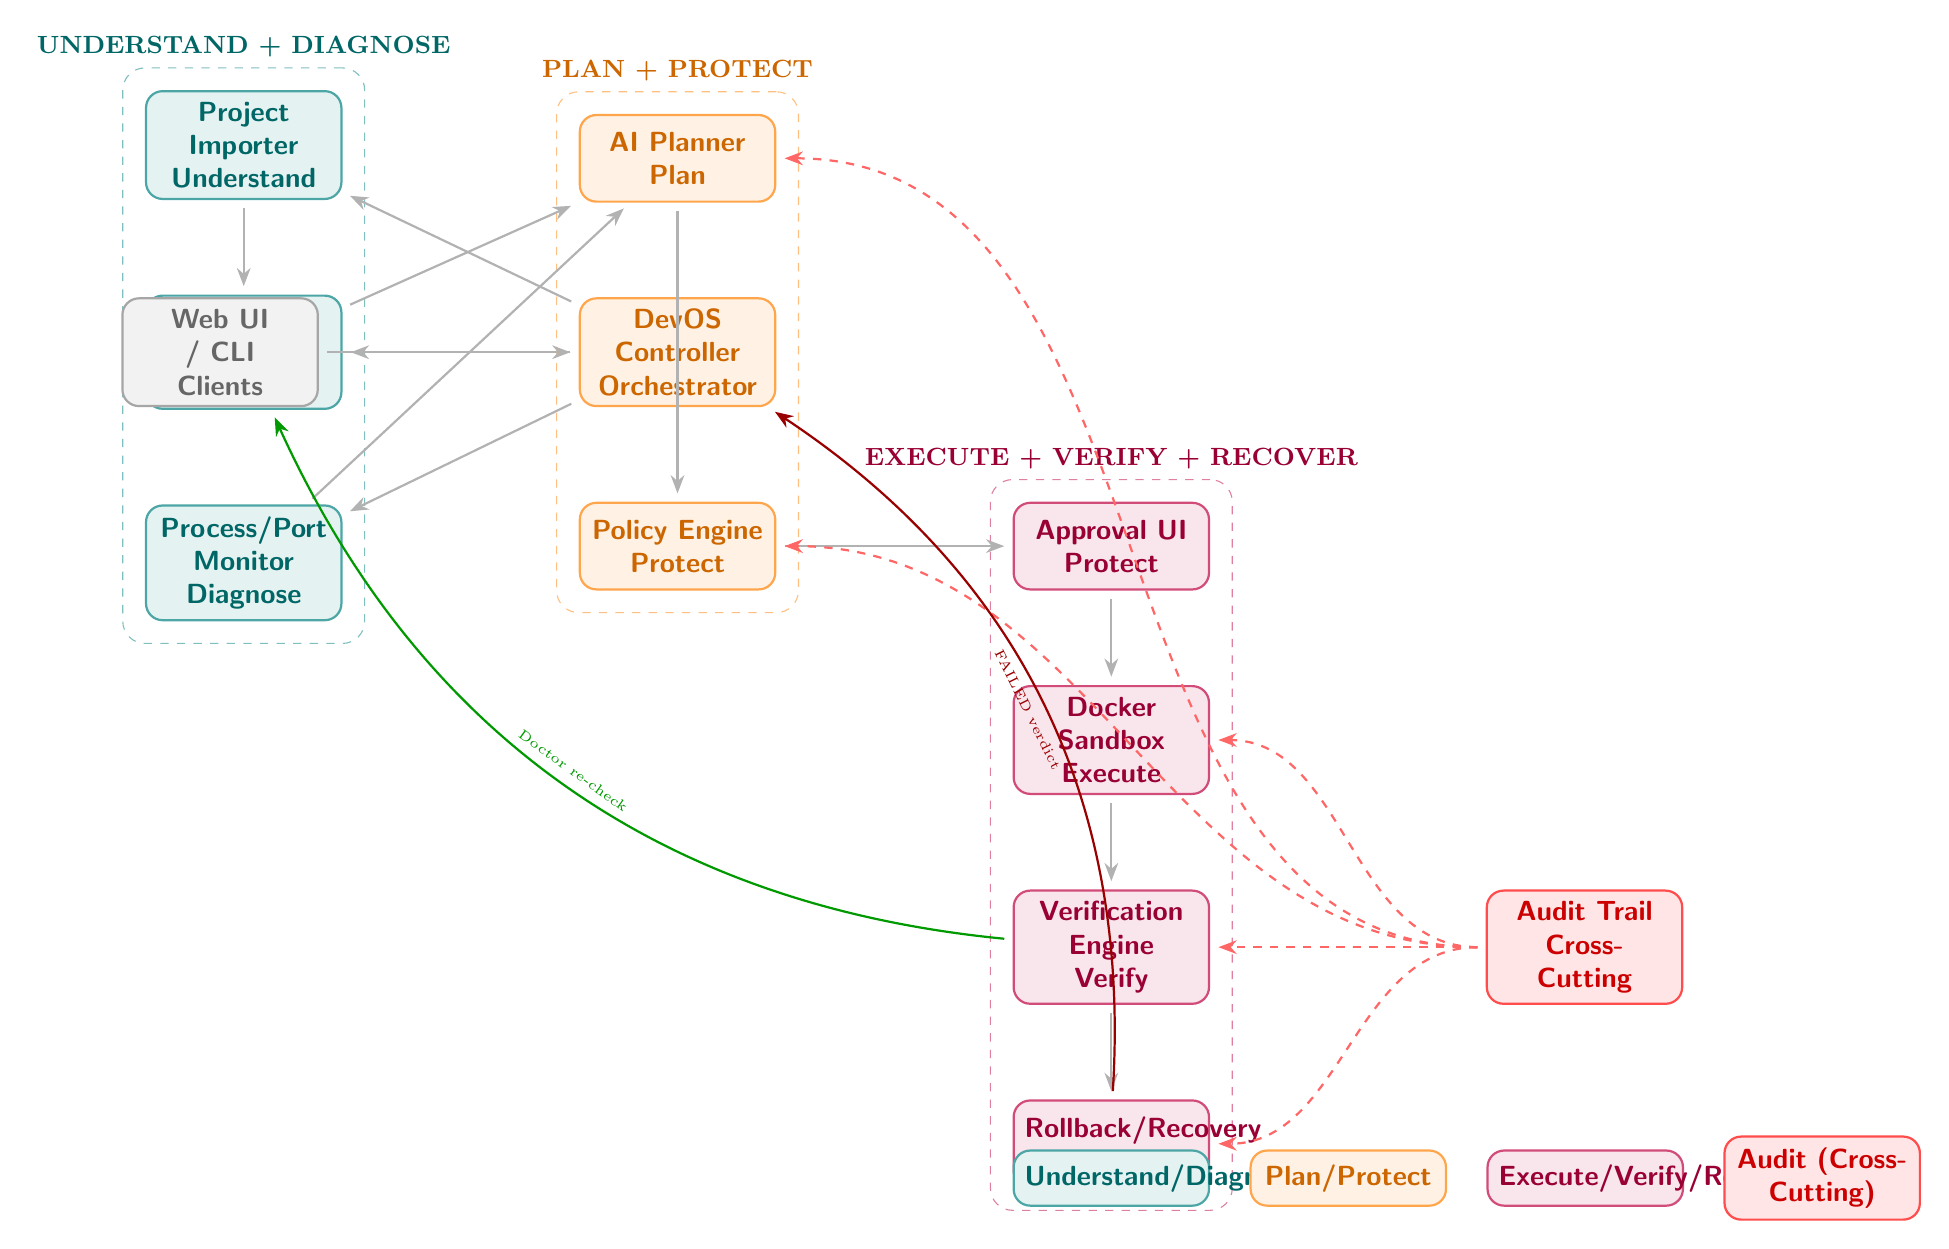
\begin{tikzpicture}[
    node distance=1.2cm and 1.5cm,
    >=Stealth,
    thick,
    font=\small,
    component/.style={
        rectangle,
        draw=#1!70,
        fill=#1!10,
        rounded corners=6pt,
        minimum height=1.1cm,
        minimum width=2.4cm,
        text centered,
        text width=2.2cm,
        inner sep=4pt
    },
    component/.default=blue,
    arrow/.style={->, thick, shorten >=3pt, shorten <=3pt, color=gray!60},
    crossarrow/.style={->, thick, dashed, shorten >=3pt, shorten <=3pt, color=red!60},
    title/.style={font=\bfseries\sffamily, text=#1!80!black},
    title/.default=blue
]

% ============================================================
% LEFT COLUMN: UNDERSTAND + DIAGNOSE
% ============================================================
\node[component=teal, title=teal] (importer) {\textbf{Project Importer}\\Understand};
\node[component=teal, title=teal, below=of importer] (doctor) {\textbf{Project Doctor}\\Diagnose};
\node[component=teal, title=teal, below=of doctor] (monitor) {\textbf{Process/Port Monitor}\\Diagnose};

% ============================================================
% CENTER: CONTROLLER + PLANNER + POLICY
% ============================================================
\node[component=orange, title=orange, right=of doctor, xshift=1.5cm] (controller) {\textbf{DevOS Controller}\\Orchestrator};
\node[component=orange, title=orange, above=of controller] (planner) {\textbf{AI Planner}\\Plan};
\node[component=orange, title=orange, below=of controller] (policy) {\textbf{Policy Engine}\\Protect};

% ============================================================
% RIGHT COLUMN: EXECUTE + VERIFY + RECOVER
% ============================================================
\node[component=purple, title=purple, right=of policy, xshift=1.5cm] (approval) {\textbf{Approval UI}\\Protect};
\node[component=purple, title=purple, below=of approval] (sandbox) {\textbf{Docker Sandbox}\\Execute};
\node[component=purple, title=purple, below=of sandbox] (verify) {\textbf{Verification Engine}\\Verify};
\node[component=purple, title=purple, below=of verify] (rollback) {\textbf{Rollback/Recovery}\\Recover};

% ============================================================
% CROSS-CUTTING: AUDIT TRAIL
% ============================================================
\node[component=red, title=red, right=of verify, xshift=2cm] (audit) {\textbf{Audit Trail}\\Cross-Cutting};

% ============================================================
% CLIENTS
% ============================================================
\node[component=gray, title=gray, left=of controller, xshift=-1.8cm] (ui) {\textbf{Web UI / CLI}\\Clients};

% ============================================================
% ARROWS: MAIN FLOW
% ============================================================
% Clients -> Controller
\draw[arrow] (ui) -- (controller);

% Controller -> Understand/Diagnose
\draw[arrow] (controller) -- (importer);
\draw[arrow] (controller) -- (doctor);
\draw[arrow] (controller) -- (monitor);

% Understand -> Diagnose -> Plan
\draw[arrow] (importer) -- (doctor);
\draw[arrow] (doctor) -- (planner);
\draw[arrow] (monitor) -- (planner);

% Plan -> Policy -> Approval -> Sandbox -> Verify -> Rollback
\draw[arrow] (planner) -- (policy);
\draw[arrow] (policy) -- (approval);
\draw[arrow] (approval) -- (sandbox);
\draw[arrow] (sandbox) -- (verify);
\draw[arrow] (verify) -- (rollback);

% ============================================================
% ARROWS: AUDIT (CROSS-CUTTING, DASHED)
% ============================================================
\draw[crossarrow] (audit) to[out=180,in=0] (verify);
\draw[crossarrow] (audit) to[out=180,in=0] (rollback);
\draw[crossarrow] (audit) to[out=180,in=0] (planner);
\draw[crossarrow] (audit) to[out=180,in=0] (policy);
\draw[crossarrow] (audit) to[out=180,in=0] (sandbox);

% ============================================================
% ARROWS: FEEDBACK LOOPS
% ============================================================
% Verification -> Doctor (re-check)
\draw[arrow, bend left=30, color=green!60!black] (verify) to node[midway, above, sloped, font=\tiny, color=green!60!black] {Doctor re-check} (doctor);

% Rollback -> Controller (on failure)
\draw[arrow, bend right=30, color=red!60!black] (rollback) to node[midway, below, sloped, font=\tiny, color=red!60!black] {FAILED verdict} (controller);

% ============================================================
% PHASE LABELS (BACKGROUND BOXES)
% ============================================================
\begin{scope}[on background layer]
  % Understand + Diagnose phase
  \node[fit=(importer)(doctor)(monitor), draw=teal!50, dashed, rounded corners=8pt, inner sep=8pt, label={[font=\bfseries\small, text=teal!80!black]above:UNDERSTAND + DIAGNOSE}] {};
  
  % Plan + Protect phase
  \node[fit=(planner)(controller)(policy), draw=orange!50, dashed, rounded corners=8pt, inner sep=8pt, label={[font=\bfseries\small, text=orange!80!black]above:PLAN + PROTECT}] {};
  
  % Execute + Verify + Recover phase
  \node[fit=(approval)(sandbox)(verify)(rollback), draw=purple!50, dashed, rounded corners=8pt, inner sep=8pt, label={[font=\bfseries\small, text=purple!80!black]above:EXECUTE + VERIFY + RECOVER}] {};
\end{scope}

% ============================================================
% LEGEND
% ============================================================
\begin{scope}[shift={($(verify.south)+(0,-2.2)$)}]
  \node[component=teal, title=teal, minimum height=0.7cm, minimum width=2cm] (l1) {Understand/Diagnose};
  \node[component=orange, title=orange, minimum height=0.7cm, minimum width=2cm, right=0.5cm of l1] (l2) {Plan/Protect};
  \node[component=purple, title=purple, minimum height=0.7cm, minimum width=2cm, right=0.5cm of l2] (l3) {Execute/Verify/Recover};
  \node[component=red, title=red, minimum height=0.7cm, minimum width=2cm, right=0.5cm of l3] (l4) {Audit (Cross-Cutting)};
\end{scope}

\end{tikzpicture}

\end{document}